\documentclass[margin=2mm]{standalone}
\usepackage{tikz}
\usepackage{amsmath,amssymb,mathtools}
\begin{document}
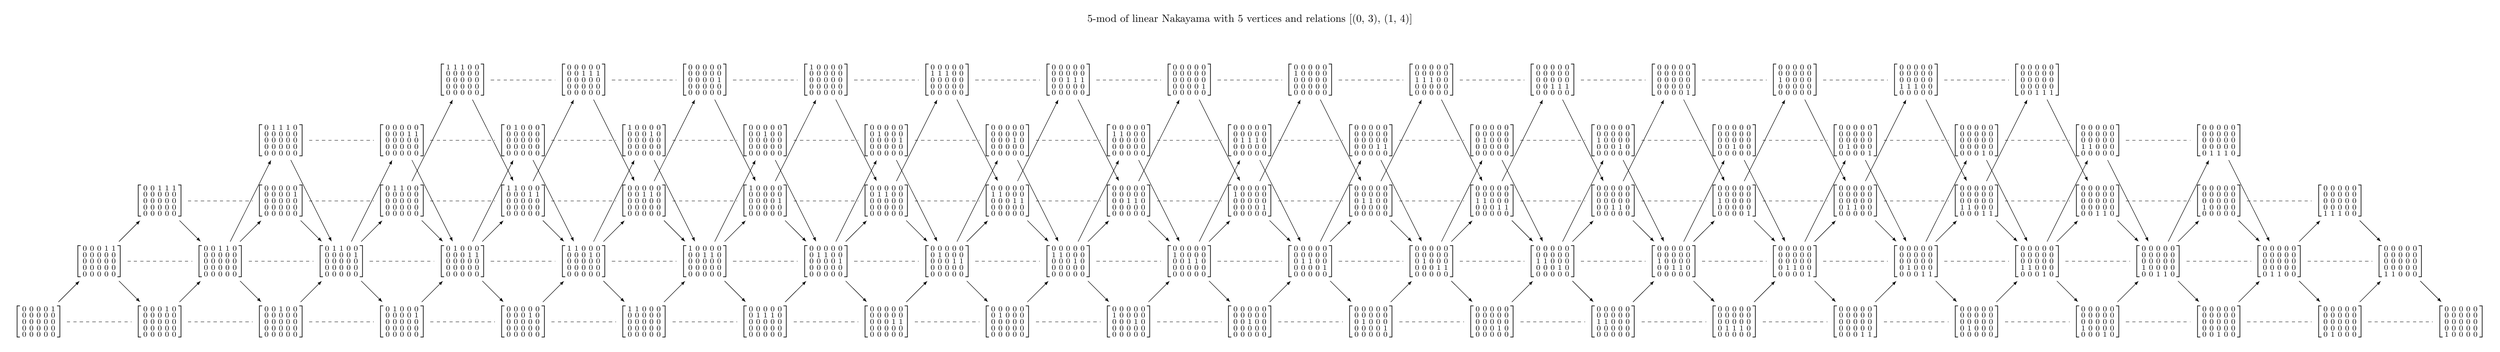
\begin{tikzpicture}[xscale=2,yscale=2]
\node at (20.0,5) [] {$5$-mod of linear Nakayama with 5 vertices and relations [(0, 3), (1, 4)]};
\node (t-0P0) at (7,4) [scale=1] {$\begin{bsmallmatrix}
 1 & 1 & 1 & 0 & 0\\
 0 & 0 & 0 & 0 & 0\\
 0 & 0 & 0 & 0 & 0\\
 0 & 0 & 0 & 0 & 0\\
 0 & 0 & 0 & 0 & 0\\
\end{bsmallmatrix}$};
\node (t-1P0) at (9,4) [scale=1] {$\begin{bsmallmatrix}
 0 & 0 & 0 & 0 & 0\\
 0 & 0 & 1 & 1 & 1\\
 0 & 0 & 0 & 0 & 0\\
 0 & 0 & 0 & 0 & 0\\
 0 & 0 & 0 & 0 & 0\\
\end{bsmallmatrix}$};
\node (t-2P0) at (11,4) [scale=1] {$\begin{bsmallmatrix}
 0 & 0 & 0 & 0 & 0\\
 0 & 0 & 0 & 0 & 0\\
 0 & 0 & 0 & 0 & 1\\
 0 & 0 & 0 & 0 & 0\\
 0 & 0 & 0 & 0 & 0\\
\end{bsmallmatrix}$};
\node (t-3P0) at (13,4) [scale=1] {$\begin{bsmallmatrix}
 1 & 0 & 0 & 0 & 0\\
 0 & 0 & 0 & 0 & 0\\
 0 & 0 & 0 & 0 & 0\\
 0 & 0 & 0 & 0 & 0\\
 0 & 0 & 0 & 0 & 0\\
\end{bsmallmatrix}$};
\node (t-4P0) at (15,4) [scale=1] {$\begin{bsmallmatrix}
 0 & 0 & 0 & 0 & 0\\
 1 & 1 & 1 & 0 & 0\\
 0 & 0 & 0 & 0 & 0\\
 0 & 0 & 0 & 0 & 0\\
 0 & 0 & 0 & 0 & 0\\
\end{bsmallmatrix}$};
\node (t-5P0) at (17,4) [scale=1] {$\begin{bsmallmatrix}
 0 & 0 & 0 & 0 & 0\\
 0 & 0 & 0 & 0 & 0\\
 0 & 0 & 1 & 1 & 1\\
 0 & 0 & 0 & 0 & 0\\
 0 & 0 & 0 & 0 & 0\\
\end{bsmallmatrix}$};
\node (t-6P0) at (19,4) [scale=1] {$\begin{bsmallmatrix}
 0 & 0 & 0 & 0 & 0\\
 0 & 0 & 0 & 0 & 0\\
 0 & 0 & 0 & 0 & 0\\
 0 & 0 & 0 & 0 & 1\\
 0 & 0 & 0 & 0 & 0\\
\end{bsmallmatrix}$};
\node (t-7P0) at (21,4) [scale=1] {$\begin{bsmallmatrix}
 0 & 0 & 0 & 0 & 0\\
 1 & 0 & 0 & 0 & 0\\
 0 & 0 & 0 & 0 & 0\\
 0 & 0 & 0 & 0 & 0\\
 0 & 0 & 0 & 0 & 0\\
\end{bsmallmatrix}$};
\node (t-8P0) at (23,4) [scale=1] {$\begin{bsmallmatrix}
 0 & 0 & 0 & 0 & 0\\
 0 & 0 & 0 & 0 & 0\\
 1 & 1 & 1 & 0 & 0\\
 0 & 0 & 0 & 0 & 0\\
 0 & 0 & 0 & 0 & 0\\
\end{bsmallmatrix}$};
\node (t-9P0) at (25,4) [scale=1] {$\begin{bsmallmatrix}
 0 & 0 & 0 & 0 & 0\\
 0 & 0 & 0 & 0 & 0\\
 0 & 0 & 0 & 0 & 0\\
 0 & 0 & 1 & 1 & 1\\
 0 & 0 & 0 & 0 & 0\\
\end{bsmallmatrix}$};
\node (t-10P0) at (27,4) [scale=1] {$\begin{bsmallmatrix}
 0 & 0 & 0 & 0 & 0\\
 0 & 0 & 0 & 0 & 0\\
 0 & 0 & 0 & 0 & 0\\
 0 & 0 & 0 & 0 & 0\\
 0 & 0 & 0 & 0 & 1\\
\end{bsmallmatrix}$};
\node (t-11P0) at (29,4) [scale=1] {$\begin{bsmallmatrix}
 0 & 0 & 0 & 0 & 0\\
 0 & 0 & 0 & 0 & 0\\
 1 & 0 & 0 & 0 & 0\\
 0 & 0 & 0 & 0 & 0\\
 0 & 0 & 0 & 0 & 0\\
\end{bsmallmatrix}$};
\node (t-12P0) at (31,4) [scale=1] {$\begin{bsmallmatrix}
 0 & 0 & 0 & 0 & 0\\
 0 & 0 & 0 & 0 & 0\\
 0 & 0 & 0 & 0 & 0\\
 1 & 1 & 1 & 0 & 0\\
 0 & 0 & 0 & 0 & 0\\
\end{bsmallmatrix}$};
\node (t-13P0) at (33,4) [scale=1] {$\begin{bsmallmatrix}
 0 & 0 & 0 & 0 & 0\\
 0 & 0 & 0 & 0 & 0\\
 0 & 0 & 0 & 0 & 0\\
 0 & 0 & 0 & 0 & 0\\
 0 & 0 & 1 & 1 & 1\\
\end{bsmallmatrix}$};
\node (t-0P1) at (4,3) [scale=1] {$\begin{bsmallmatrix}
 0 & 1 & 1 & 1 & 0\\
 0 & 0 & 0 & 0 & 0\\
 0 & 0 & 0 & 0 & 0\\
 0 & 0 & 0 & 0 & 0\\
 0 & 0 & 0 & 0 & 0\\
\end{bsmallmatrix}$};
\node (t-1P1) at (6,3) [scale=1] {$\begin{bsmallmatrix}
 0 & 0 & 0 & 0 & 0\\
 0 & 0 & 0 & 1 & 1\\
 0 & 0 & 0 & 0 & 0\\
 0 & 0 & 0 & 0 & 0\\
 0 & 0 & 0 & 0 & 0\\
\end{bsmallmatrix}$};
\node (t-2P1) at (8,3) [scale=1] {$\begin{bsmallmatrix}
 0 & 1 & 0 & 0 & 0\\
 0 & 0 & 0 & 0 & 0\\
 0 & 0 & 0 & 0 & 0\\
 0 & 0 & 0 & 0 & 0\\
 0 & 0 & 0 & 0 & 0\\
\end{bsmallmatrix}$};
\node (t-3P1) at (10,3) [scale=1] {$\begin{bsmallmatrix}
 1 & 0 & 0 & 0 & 0\\
 0 & 0 & 0 & 1 & 0\\
 0 & 0 & 0 & 0 & 0\\
 0 & 0 & 0 & 0 & 0\\
 0 & 0 & 0 & 0 & 0\\
\end{bsmallmatrix}$};
\node (t-4P1) at (12,3) [scale=1] {$\begin{bsmallmatrix}
 0 & 0 & 0 & 0 & 0\\
 0 & 0 & 1 & 0 & 0\\
 0 & 0 & 0 & 0 & 0\\
 0 & 0 & 0 & 0 & 0\\
 0 & 0 & 0 & 0 & 0\\
\end{bsmallmatrix}$};
\node (t-5P1) at (14,3) [scale=1] {$\begin{bsmallmatrix}
 0 & 0 & 0 & 0 & 0\\
 0 & 1 & 0 & 0 & 0\\
 0 & 0 & 0 & 0 & 1\\
 0 & 0 & 0 & 0 & 0\\
 0 & 0 & 0 & 0 & 0\\
\end{bsmallmatrix}$};
\node (t-6P1) at (16,3) [scale=1] {$\begin{bsmallmatrix}
 0 & 0 & 0 & 0 & 0\\
 0 & 0 & 0 & 0 & 0\\
 0 & 0 & 0 & 1 & 0\\
 0 & 0 & 0 & 0 & 0\\
 0 & 0 & 0 & 0 & 0\\
\end{bsmallmatrix}$};
\node (t-7P1) at (18,3) [scale=1] {$\begin{bsmallmatrix}
 0 & 0 & 0 & 0 & 0\\
 1 & 1 & 0 & 0 & 0\\
 0 & 0 & 0 & 0 & 0\\
 0 & 0 & 0 & 0 & 0\\
 0 & 0 & 0 & 0 & 0\\
\end{bsmallmatrix}$};
\node (t-8P1) at (20,3) [scale=1] {$\begin{bsmallmatrix}
 0 & 0 & 0 & 0 & 0\\
 0 & 0 & 0 & 0 & 0\\
 0 & 1 & 1 & 1 & 0\\
 0 & 0 & 0 & 0 & 0\\
 0 & 0 & 0 & 0 & 0\\
\end{bsmallmatrix}$};
\node (t-9P1) at (22,3) [scale=1] {$\begin{bsmallmatrix}
 0 & 0 & 0 & 0 & 0\\
 0 & 0 & 0 & 0 & 0\\
 0 & 0 & 0 & 0 & 0\\
 0 & 0 & 0 & 1 & 1\\
 0 & 0 & 0 & 0 & 0\\
\end{bsmallmatrix}$};
\node (t-10P1) at (24,3) [scale=1] {$\begin{bsmallmatrix}
 0 & 0 & 0 & 0 & 0\\
 0 & 0 & 0 & 0 & 0\\
 0 & 1 & 0 & 0 & 0\\
 0 & 0 & 0 & 0 & 0\\
 0 & 0 & 0 & 0 & 0\\
\end{bsmallmatrix}$};
\node (t-11P1) at (26,3) [scale=1] {$\begin{bsmallmatrix}
 0 & 0 & 0 & 0 & 0\\
 0 & 0 & 0 & 0 & 0\\
 1 & 0 & 0 & 0 & 0\\
 0 & 0 & 0 & 1 & 0\\
 0 & 0 & 0 & 0 & 0\\
\end{bsmallmatrix}$};
\node (t-12P1) at (28,3) [scale=1] {$\begin{bsmallmatrix}
 0 & 0 & 0 & 0 & 0\\
 0 & 0 & 0 & 0 & 0\\
 0 & 0 & 0 & 0 & 0\\
 0 & 0 & 1 & 0 & 0\\
 0 & 0 & 0 & 0 & 0\\
\end{bsmallmatrix}$};
\node (t-13P1) at (30,3) [scale=1] {$\begin{bsmallmatrix}
 0 & 0 & 0 & 0 & 0\\
 0 & 0 & 0 & 0 & 0\\
 0 & 0 & 0 & 0 & 0\\
 0 & 1 & 0 & 0 & 0\\
 0 & 0 & 0 & 0 & 1\\
\end{bsmallmatrix}$};
\node (t-14P1) at (32,3) [scale=1] {$\begin{bsmallmatrix}
 0 & 0 & 0 & 0 & 0\\
 0 & 0 & 0 & 0 & 0\\
 0 & 0 & 0 & 0 & 0\\
 0 & 0 & 0 & 0 & 0\\
 0 & 0 & 0 & 1 & 0\\
\end{bsmallmatrix}$};
\node (t-15P1) at (34,3) [scale=1] {$\begin{bsmallmatrix}
 0 & 0 & 0 & 0 & 0\\
 0 & 0 & 0 & 0 & 0\\
 0 & 0 & 0 & 0 & 0\\
 1 & 1 & 0 & 0 & 0\\
 0 & 0 & 0 & 0 & 0\\
\end{bsmallmatrix}$};
\node (t-16P1) at (36,3) [scale=1] {$\begin{bsmallmatrix}
 0 & 0 & 0 & 0 & 0\\
 0 & 0 & 0 & 0 & 0\\
 0 & 0 & 0 & 0 & 0\\
 0 & 0 & 0 & 0 & 0\\
 0 & 1 & 1 & 1 & 0\\
\end{bsmallmatrix}$};
\node (t-0P2) at (2,2) [scale=1] {$\begin{bsmallmatrix}
 0 & 0 & 1 & 1 & 1\\
 0 & 0 & 0 & 0 & 0\\
 0 & 0 & 0 & 0 & 0\\
 0 & 0 & 0 & 0 & 0\\
 0 & 0 & 0 & 0 & 0\\
\end{bsmallmatrix}$};
\node (t-1P2) at (4,2) [scale=1] {$\begin{bsmallmatrix}
 0 & 0 & 0 & 0 & 0\\
 0 & 0 & 0 & 0 & 1\\
 0 & 0 & 0 & 0 & 0\\
 0 & 0 & 0 & 0 & 0\\
 0 & 0 & 0 & 0 & 0\\
\end{bsmallmatrix}$};
\node (t-2P2) at (6,2) [scale=1] {$\begin{bsmallmatrix}
 0 & 1 & 1 & 0 & 0\\
 0 & 0 & 0 & 0 & 0\\
 0 & 0 & 0 & 0 & 0\\
 0 & 0 & 0 & 0 & 0\\
 0 & 0 & 0 & 0 & 0\\
\end{bsmallmatrix}$};
\node (t-3P2) at (8,2) [scale=1] {$\begin{bsmallmatrix}
 1 & 1 & 0 & 0 & 0\\
 0 & 0 & 0 & 1 & 1\\
 0 & 0 & 0 & 0 & 0\\
 0 & 0 & 0 & 0 & 0\\
 0 & 0 & 0 & 0 & 0\\
\end{bsmallmatrix}$};
\node (t-4P2) at (10,2) [scale=1] {$\begin{bsmallmatrix}
 0 & 0 & 0 & 0 & 0\\
 0 & 0 & 1 & 1 & 0\\
 0 & 0 & 0 & 0 & 0\\
 0 & 0 & 0 & 0 & 0\\
 0 & 0 & 0 & 0 & 0\\
\end{bsmallmatrix}$};
\node (t-5P2) at (12,2) [scale=1] {$\begin{bsmallmatrix}
 1 & 0 & 0 & 0 & 0\\
 0 & 0 & 0 & 0 & 0\\
 0 & 0 & 0 & 0 & 1\\
 0 & 0 & 0 & 0 & 0\\
 0 & 0 & 0 & 0 & 0\\
\end{bsmallmatrix}$};
\node (t-6P2) at (14,2) [scale=1] {$\begin{bsmallmatrix}
 0 & 0 & 0 & 0 & 0\\
 0 & 1 & 1 & 0 & 0\\
 0 & 0 & 0 & 0 & 0\\
 0 & 0 & 0 & 0 & 0\\
 0 & 0 & 0 & 0 & 0\\
\end{bsmallmatrix}$};
\node (t-7P2) at (16,2) [scale=1] {$\begin{bsmallmatrix}
 0 & 0 & 0 & 0 & 0\\
 1 & 1 & 0 & 0 & 0\\
 0 & 0 & 0 & 1 & 1\\
 0 & 0 & 0 & 0 & 0\\
 0 & 0 & 0 & 0 & 0\\
\end{bsmallmatrix}$};
\node (t-8P2) at (18,2) [scale=1] {$\begin{bsmallmatrix}
 0 & 0 & 0 & 0 & 0\\
 0 & 0 & 0 & 0 & 0\\
 0 & 0 & 1 & 1 & 0\\
 0 & 0 & 0 & 0 & 0\\
 0 & 0 & 0 & 0 & 0\\
\end{bsmallmatrix}$};
\node (t-9P2) at (20,2) [scale=1] {$\begin{bsmallmatrix}
 0 & 0 & 0 & 0 & 0\\
 1 & 0 & 0 & 0 & 0\\
 0 & 0 & 0 & 0 & 0\\
 0 & 0 & 0 & 0 & 1\\
 0 & 0 & 0 & 0 & 0\\
\end{bsmallmatrix}$};
\node (t-10P2) at (22,2) [scale=1] {$\begin{bsmallmatrix}
 0 & 0 & 0 & 0 & 0\\
 0 & 0 & 0 & 0 & 0\\
 0 & 1 & 1 & 0 & 0\\
 0 & 0 & 0 & 0 & 0\\
 0 & 0 & 0 & 0 & 0\\
\end{bsmallmatrix}$};
\node (t-11P2) at (24,2) [scale=1] {$\begin{bsmallmatrix}
 0 & 0 & 0 & 0 & 0\\
 0 & 0 & 0 & 0 & 0\\
 1 & 1 & 0 & 0 & 0\\
 0 & 0 & 0 & 1 & 1\\
 0 & 0 & 0 & 0 & 0\\
\end{bsmallmatrix}$};
\node (t-12P2) at (26,2) [scale=1] {$\begin{bsmallmatrix}
 0 & 0 & 0 & 0 & 0\\
 0 & 0 & 0 & 0 & 0\\
 0 & 0 & 0 & 0 & 0\\
 0 & 0 & 1 & 1 & 0\\
 0 & 0 & 0 & 0 & 0\\
\end{bsmallmatrix}$};
\node (t-13P2) at (28,2) [scale=1] {$\begin{bsmallmatrix}
 0 & 0 & 0 & 0 & 0\\
 0 & 0 & 0 & 0 & 0\\
 1 & 0 & 0 & 0 & 0\\
 0 & 0 & 0 & 0 & 0\\
 0 & 0 & 0 & 0 & 1\\
\end{bsmallmatrix}$};
\node (t-14P2) at (30,2) [scale=1] {$\begin{bsmallmatrix}
 0 & 0 & 0 & 0 & 0\\
 0 & 0 & 0 & 0 & 0\\
 0 & 0 & 0 & 0 & 0\\
 0 & 1 & 1 & 0 & 0\\
 0 & 0 & 0 & 0 & 0\\
\end{bsmallmatrix}$};
\node (t-15P2) at (32,2) [scale=1] {$\begin{bsmallmatrix}
 0 & 0 & 0 & 0 & 0\\
 0 & 0 & 0 & 0 & 0\\
 0 & 0 & 0 & 0 & 0\\
 1 & 1 & 0 & 0 & 0\\
 0 & 0 & 0 & 1 & 1\\
\end{bsmallmatrix}$};
\node (t-16P2) at (34,2) [scale=1] {$\begin{bsmallmatrix}
 0 & 0 & 0 & 0 & 0\\
 0 & 0 & 0 & 0 & 0\\
 0 & 0 & 0 & 0 & 0\\
 0 & 0 & 0 & 0 & 0\\
 0 & 0 & 1 & 1 & 0\\
\end{bsmallmatrix}$};
\node (t-17P2) at (36,2) [scale=1] {$\begin{bsmallmatrix}
 0 & 0 & 0 & 0 & 0\\
 0 & 0 & 0 & 0 & 0\\
 0 & 0 & 0 & 0 & 0\\
 1 & 0 & 0 & 0 & 0\\
 0 & 0 & 0 & 0 & 0\\
\end{bsmallmatrix}$};
\node (t-18P2) at (38,2) [scale=1] {$\begin{bsmallmatrix}
 0 & 0 & 0 & 0 & 0\\
 0 & 0 & 0 & 0 & 0\\
 0 & 0 & 0 & 0 & 0\\
 0 & 0 & 0 & 0 & 0\\
 1 & 1 & 1 & 0 & 0\\
\end{bsmallmatrix}$};
\node (t-0P3) at (1,1) [scale=1] {$\begin{bsmallmatrix}
 0 & 0 & 0 & 1 & 1\\
 0 & 0 & 0 & 0 & 0\\
 0 & 0 & 0 & 0 & 0\\
 0 & 0 & 0 & 0 & 0\\
 0 & 0 & 0 & 0 & 0\\
\end{bsmallmatrix}$};
\node (t-1P3) at (3,1) [scale=1] {$\begin{bsmallmatrix}
 0 & 0 & 1 & 1 & 0\\
 0 & 0 & 0 & 0 & 0\\
 0 & 0 & 0 & 0 & 0\\
 0 & 0 & 0 & 0 & 0\\
 0 & 0 & 0 & 0 & 0\\
\end{bsmallmatrix}$};
\node (t-2P3) at (5,1) [scale=1] {$\begin{bsmallmatrix}
 0 & 1 & 1 & 0 & 0\\
 0 & 0 & 0 & 0 & 1\\
 0 & 0 & 0 & 0 & 0\\
 0 & 0 & 0 & 0 & 0\\
 0 & 0 & 0 & 0 & 0\\
\end{bsmallmatrix}$};
\node (t-3P3) at (7,1) [scale=1] {$\begin{bsmallmatrix}
 0 & 1 & 0 & 0 & 0\\
 0 & 0 & 0 & 1 & 1\\
 0 & 0 & 0 & 0 & 0\\
 0 & 0 & 0 & 0 & 0\\
 0 & 0 & 0 & 0 & 0\\
\end{bsmallmatrix}$};
\node (t-4P3) at (9,1) [scale=1] {$\begin{bsmallmatrix}
 1 & 1 & 0 & 0 & 0\\
 0 & 0 & 0 & 1 & 0\\
 0 & 0 & 0 & 0 & 0\\
 0 & 0 & 0 & 0 & 0\\
 0 & 0 & 0 & 0 & 0\\
\end{bsmallmatrix}$};
\node (t-5P3) at (11,1) [scale=1] {$\begin{bsmallmatrix}
 1 & 0 & 0 & 0 & 0\\
 0 & 0 & 1 & 1 & 0\\
 0 & 0 & 0 & 0 & 0\\
 0 & 0 & 0 & 0 & 0\\
 0 & 0 & 0 & 0 & 0\\
\end{bsmallmatrix}$};
\node (t-6P3) at (13,1) [scale=1] {$\begin{bsmallmatrix}
 0 & 0 & 0 & 0 & 0\\
 0 & 1 & 1 & 0 & 0\\
 0 & 0 & 0 & 0 & 1\\
 0 & 0 & 0 & 0 & 0\\
 0 & 0 & 0 & 0 & 0\\
\end{bsmallmatrix}$};
\node (t-7P3) at (15,1) [scale=1] {$\begin{bsmallmatrix}
 0 & 0 & 0 & 0 & 0\\
 0 & 1 & 0 & 0 & 0\\
 0 & 0 & 0 & 1 & 1\\
 0 & 0 & 0 & 0 & 0\\
 0 & 0 & 0 & 0 & 0\\
\end{bsmallmatrix}$};
\node (t-8P3) at (17,1) [scale=1] {$\begin{bsmallmatrix}
 0 & 0 & 0 & 0 & 0\\
 1 & 1 & 0 & 0 & 0\\
 0 & 0 & 0 & 1 & 0\\
 0 & 0 & 0 & 0 & 0\\
 0 & 0 & 0 & 0 & 0\\
\end{bsmallmatrix}$};
\node (t-9P3) at (19,1) [scale=1] {$\begin{bsmallmatrix}
 0 & 0 & 0 & 0 & 0\\
 1 & 0 & 0 & 0 & 0\\
 0 & 0 & 1 & 1 & 0\\
 0 & 0 & 0 & 0 & 0\\
 0 & 0 & 0 & 0 & 0\\
\end{bsmallmatrix}$};
\node (t-10P3) at (21,1) [scale=1] {$\begin{bsmallmatrix}
 0 & 0 & 0 & 0 & 0\\
 0 & 0 & 0 & 0 & 0\\
 0 & 1 & 1 & 0 & 0\\
 0 & 0 & 0 & 0 & 1\\
 0 & 0 & 0 & 0 & 0\\
\end{bsmallmatrix}$};
\node (t-11P3) at (23,1) [scale=1] {$\begin{bsmallmatrix}
 0 & 0 & 0 & 0 & 0\\
 0 & 0 & 0 & 0 & 0\\
 0 & 1 & 0 & 0 & 0\\
 0 & 0 & 0 & 1 & 1\\
 0 & 0 & 0 & 0 & 0\\
\end{bsmallmatrix}$};
\node (t-12P3) at (25,1) [scale=1] {$\begin{bsmallmatrix}
 0 & 0 & 0 & 0 & 0\\
 0 & 0 & 0 & 0 & 0\\
 1 & 1 & 0 & 0 & 0\\
 0 & 0 & 0 & 1 & 0\\
 0 & 0 & 0 & 0 & 0\\
\end{bsmallmatrix}$};
\node (t-13P3) at (27,1) [scale=1] {$\begin{bsmallmatrix}
 0 & 0 & 0 & 0 & 0\\
 0 & 0 & 0 & 0 & 0\\
 1 & 0 & 0 & 0 & 0\\
 0 & 0 & 1 & 1 & 0\\
 0 & 0 & 0 & 0 & 0\\
\end{bsmallmatrix}$};
\node (t-14P3) at (29,1) [scale=1] {$\begin{bsmallmatrix}
 0 & 0 & 0 & 0 & 0\\
 0 & 0 & 0 & 0 & 0\\
 0 & 0 & 0 & 0 & 0\\
 0 & 1 & 1 & 0 & 0\\
 0 & 0 & 0 & 0 & 1\\
\end{bsmallmatrix}$};
\node (t-15P3) at (31,1) [scale=1] {$\begin{bsmallmatrix}
 0 & 0 & 0 & 0 & 0\\
 0 & 0 & 0 & 0 & 0\\
 0 & 0 & 0 & 0 & 0\\
 0 & 1 & 0 & 0 & 0\\
 0 & 0 & 0 & 1 & 1\\
\end{bsmallmatrix}$};
\node (t-16P3) at (33,1) [scale=1] {$\begin{bsmallmatrix}
 0 & 0 & 0 & 0 & 0\\
 0 & 0 & 0 & 0 & 0\\
 0 & 0 & 0 & 0 & 0\\
 1 & 1 & 0 & 0 & 0\\
 0 & 0 & 0 & 1 & 0\\
\end{bsmallmatrix}$};
\node (t-17P3) at (35,1) [scale=1] {$\begin{bsmallmatrix}
 0 & 0 & 0 & 0 & 0\\
 0 & 0 & 0 & 0 & 0\\
 0 & 0 & 0 & 0 & 0\\
 1 & 0 & 0 & 0 & 0\\
 0 & 0 & 1 & 1 & 0\\
\end{bsmallmatrix}$};
\node (t-18P3) at (37,1) [scale=1] {$\begin{bsmallmatrix}
 0 & 0 & 0 & 0 & 0\\
 0 & 0 & 0 & 0 & 0\\
 0 & 0 & 0 & 0 & 0\\
 0 & 0 & 0 & 0 & 0\\
 0 & 1 & 1 & 0 & 0\\
\end{bsmallmatrix}$};
\node (t-19P3) at (39,1) [scale=1] {$\begin{bsmallmatrix}
 0 & 0 & 0 & 0 & 0\\
 0 & 0 & 0 & 0 & 0\\
 0 & 0 & 0 & 0 & 0\\
 0 & 0 & 0 & 0 & 0\\
 1 & 1 & 0 & 0 & 0\\
\end{bsmallmatrix}$};
\node (t-0P4) at (0,0) [scale=1] {$\begin{bsmallmatrix}
 0 & 0 & 0 & 0 & 1\\
 0 & 0 & 0 & 0 & 0\\
 0 & 0 & 0 & 0 & 0\\
 0 & 0 & 0 & 0 & 0\\
 0 & 0 & 0 & 0 & 0\\
\end{bsmallmatrix}$};
\node (t-1P4) at (2,0) [scale=1] {$\begin{bsmallmatrix}
 0 & 0 & 0 & 1 & 0\\
 0 & 0 & 0 & 0 & 0\\
 0 & 0 & 0 & 0 & 0\\
 0 & 0 & 0 & 0 & 0\\
 0 & 0 & 0 & 0 & 0\\
\end{bsmallmatrix}$};
\node (t-2P4) at (4,0) [scale=1] {$\begin{bsmallmatrix}
 0 & 0 & 1 & 0 & 0\\
 0 & 0 & 0 & 0 & 0\\
 0 & 0 & 0 & 0 & 0\\
 0 & 0 & 0 & 0 & 0\\
 0 & 0 & 0 & 0 & 0\\
\end{bsmallmatrix}$};
\node (t-3P4) at (6,0) [scale=1] {$\begin{bsmallmatrix}
 0 & 1 & 0 & 0 & 0\\
 0 & 0 & 0 & 0 & 1\\
 0 & 0 & 0 & 0 & 0\\
 0 & 0 & 0 & 0 & 0\\
 0 & 0 & 0 & 0 & 0\\
\end{bsmallmatrix}$};
\node (t-4P4) at (8,0) [scale=1] {$\begin{bsmallmatrix}
 0 & 0 & 0 & 0 & 0\\
 0 & 0 & 0 & 1 & 0\\
 0 & 0 & 0 & 0 & 0\\
 0 & 0 & 0 & 0 & 0\\
 0 & 0 & 0 & 0 & 0\\
\end{bsmallmatrix}$};
\node (t-5P4) at (10,0) [scale=1] {$\begin{bsmallmatrix}
 1 & 1 & 0 & 0 & 0\\
 0 & 0 & 0 & 0 & 0\\
 0 & 0 & 0 & 0 & 0\\
 0 & 0 & 0 & 0 & 0\\
 0 & 0 & 0 & 0 & 0\\
\end{bsmallmatrix}$};
\node (t-6P4) at (12,0) [scale=1] {$\begin{bsmallmatrix}
 0 & 0 & 0 & 0 & 0\\
 0 & 1 & 1 & 1 & 0\\
 0 & 0 & 0 & 0 & 0\\
 0 & 0 & 0 & 0 & 0\\
 0 & 0 & 0 & 0 & 0\\
\end{bsmallmatrix}$};
\node (t-7P4) at (14,0) [scale=1] {$\begin{bsmallmatrix}
 0 & 0 & 0 & 0 & 0\\
 0 & 0 & 0 & 0 & 0\\
 0 & 0 & 0 & 1 & 1\\
 0 & 0 & 0 & 0 & 0\\
 0 & 0 & 0 & 0 & 0\\
\end{bsmallmatrix}$};
\node (t-8P4) at (16,0) [scale=1] {$\begin{bsmallmatrix}
 0 & 0 & 0 & 0 & 0\\
 0 & 1 & 0 & 0 & 0\\
 0 & 0 & 0 & 0 & 0\\
 0 & 0 & 0 & 0 & 0\\
 0 & 0 & 0 & 0 & 0\\
\end{bsmallmatrix}$};
\node (t-9P4) at (18,0) [scale=1] {$\begin{bsmallmatrix}
 0 & 0 & 0 & 0 & 0\\
 1 & 0 & 0 & 0 & 0\\
 0 & 0 & 0 & 1 & 0\\
 0 & 0 & 0 & 0 & 0\\
 0 & 0 & 0 & 0 & 0\\
\end{bsmallmatrix}$};
\node (t-10P4) at (20,0) [scale=1] {$\begin{bsmallmatrix}
 0 & 0 & 0 & 0 & 0\\
 0 & 0 & 0 & 0 & 0\\
 0 & 0 & 1 & 0 & 0\\
 0 & 0 & 0 & 0 & 0\\
 0 & 0 & 0 & 0 & 0\\
\end{bsmallmatrix}$};
\node (t-11P4) at (22,0) [scale=1] {$\begin{bsmallmatrix}
 0 & 0 & 0 & 0 & 0\\
 0 & 0 & 0 & 0 & 0\\
 0 & 1 & 0 & 0 & 0\\
 0 & 0 & 0 & 0 & 1\\
 0 & 0 & 0 & 0 & 0\\
\end{bsmallmatrix}$};
\node (t-12P4) at (24,0) [scale=1] {$\begin{bsmallmatrix}
 0 & 0 & 0 & 0 & 0\\
 0 & 0 & 0 & 0 & 0\\
 0 & 0 & 0 & 0 & 0\\
 0 & 0 & 0 & 1 & 0\\
 0 & 0 & 0 & 0 & 0\\
\end{bsmallmatrix}$};
\node (t-13P4) at (26,0) [scale=1] {$\begin{bsmallmatrix}
 0 & 0 & 0 & 0 & 0\\
 0 & 0 & 0 & 0 & 0\\
 1 & 1 & 0 & 0 & 0\\
 0 & 0 & 0 & 0 & 0\\
 0 & 0 & 0 & 0 & 0\\
\end{bsmallmatrix}$};
\node (t-14P4) at (28,0) [scale=1] {$\begin{bsmallmatrix}
 0 & 0 & 0 & 0 & 0\\
 0 & 0 & 0 & 0 & 0\\
 0 & 0 & 0 & 0 & 0\\
 0 & 1 & 1 & 1 & 0\\
 0 & 0 & 0 & 0 & 0\\
\end{bsmallmatrix}$};
\node (t-15P4) at (30,0) [scale=1] {$\begin{bsmallmatrix}
 0 & 0 & 0 & 0 & 0\\
 0 & 0 & 0 & 0 & 0\\
 0 & 0 & 0 & 0 & 0\\
 0 & 0 & 0 & 0 & 0\\
 0 & 0 & 0 & 1 & 1\\
\end{bsmallmatrix}$};
\node (t-16P4) at (32,0) [scale=1] {$\begin{bsmallmatrix}
 0 & 0 & 0 & 0 & 0\\
 0 & 0 & 0 & 0 & 0\\
 0 & 0 & 0 & 0 & 0\\
 0 & 1 & 0 & 0 & 0\\
 0 & 0 & 0 & 0 & 0\\
\end{bsmallmatrix}$};
\node (t-17P4) at (34,0) [scale=1] {$\begin{bsmallmatrix}
 0 & 0 & 0 & 0 & 0\\
 0 & 0 & 0 & 0 & 0\\
 0 & 0 & 0 & 0 & 0\\
 1 & 0 & 0 & 0 & 0\\
 0 & 0 & 0 & 1 & 0\\
\end{bsmallmatrix}$};
\node (t-18P4) at (36,0) [scale=1] {$\begin{bsmallmatrix}
 0 & 0 & 0 & 0 & 0\\
 0 & 0 & 0 & 0 & 0\\
 0 & 0 & 0 & 0 & 0\\
 0 & 0 & 0 & 0 & 0\\
 0 & 0 & 1 & 0 & 0\\
\end{bsmallmatrix}$};
\node (t-19P4) at (38,0) [scale=1] {$\begin{bsmallmatrix}
 0 & 0 & 0 & 0 & 0\\
 0 & 0 & 0 & 0 & 0\\
 0 & 0 & 0 & 0 & 0\\
 0 & 0 & 0 & 0 & 0\\
 0 & 1 & 0 & 0 & 0\\
\end{bsmallmatrix}$};
\node (t-20P4) at (40,0) [scale=1] {$\begin{bsmallmatrix}
 0 & 0 & 0 & 0 & 0\\
 0 & 0 & 0 & 0 & 0\\
 0 & 0 & 0 & 0 & 0\\
 0 & 0 & 0 & 0 & 0\\
 1 & 0 & 0 & 0 & 0\\
\end{bsmallmatrix}$};
\draw[-latex] (t-0P0) -- (t-3P2);
\draw[-latex] (t-1P0) -- (t-4P2);
\draw[-latex] (t-2P0) -- (t-5P2);
\draw[-latex] (t-3P0) -- (t-6P2);
\draw[-latex] (t-4P0) -- (t-7P2);
\draw[-latex] (t-5P0) -- (t-8P2);
\draw[-latex] (t-6P0) -- (t-9P2);
\draw[-latex] (t-7P0) -- (t-10P2);
\draw[-latex] (t-8P0) -- (t-11P2);
\draw[-latex] (t-9P0) -- (t-12P2);
\draw[-latex] (t-10P0) -- (t-13P2);
\draw[-latex] (t-11P0) -- (t-14P2);
\draw[-latex] (t-12P0) -- (t-15P2);
\draw[-latex] (t-13P0) -- (t-16P2);
\draw[-latex] (t-0P1) -- (t-2P3);
\draw[-latex] (t-1P1) -- (t-3P3);
\draw[-latex] (t-2P1) -- (t-4P3);
\draw[-latex] (t-3P1) -- (t-5P3);
\draw[-latex] (t-4P1) -- (t-6P3);
\draw[-latex] (t-5P1) -- (t-7P3);
\draw[-latex] (t-6P1) -- (t-8P3);
\draw[-latex] (t-7P1) -- (t-9P3);
\draw[-latex] (t-8P1) -- (t-10P3);
\draw[-latex] (t-9P1) -- (t-11P3);
\draw[-latex] (t-10P1) -- (t-12P3);
\draw[-latex] (t-11P1) -- (t-13P3);
\draw[-latex] (t-12P1) -- (t-14P3);
\draw[-latex] (t-13P1) -- (t-15P3);
\draw[-latex] (t-14P1) -- (t-16P3);
\draw[-latex] (t-15P1) -- (t-17P3);
\draw[-latex] (t-16P1) -- (t-18P3);
\draw[-latex] (t-0P2) -- (t-1P3);
\draw[-latex] (t-1P2) -- (t-2P3);
\draw[-latex] (t-2P2) -- (t-0P0);
\draw[-latex] (t-2P2) -- (t-3P3);
\draw[-latex] (t-3P2) -- (t-4P3);
\draw[-latex] (t-3P2) -- (t-1P0);
\draw[-latex] (t-4P2) -- (t-5P3);
\draw[-latex] (t-4P2) -- (t-2P0);
\draw[-latex] (t-5P2) -- (t-6P3);
\draw[-latex] (t-5P2) -- (t-3P0);
\draw[-latex] (t-6P2) -- (t-7P3);
\draw[-latex] (t-6P2) -- (t-4P0);
\draw[-latex] (t-7P2) -- (t-8P3);
\draw[-latex] (t-7P2) -- (t-5P0);
\draw[-latex] (t-8P2) -- (t-9P3);
\draw[-latex] (t-8P2) -- (t-6P0);
\draw[-latex] (t-9P2) -- (t-10P3);
\draw[-latex] (t-9P2) -- (t-7P0);
\draw[-latex] (t-10P2) -- (t-11P3);
\draw[-latex] (t-10P2) -- (t-8P0);
\draw[-latex] (t-11P2) -- (t-12P3);
\draw[-latex] (t-11P2) -- (t-9P0);
\draw[-latex] (t-12P2) -- (t-13P3);
\draw[-latex] (t-12P2) -- (t-10P0);
\draw[-latex] (t-13P2) -- (t-14P3);
\draw[-latex] (t-13P2) -- (t-11P0);
\draw[-latex] (t-14P2) -- (t-15P3);
\draw[-latex] (t-14P2) -- (t-12P0);
\draw[-latex] (t-15P2) -- (t-16P3);
\draw[-latex] (t-15P2) -- (t-13P0);
\draw[-latex] (t-16P2) -- (t-17P3);
\draw[-latex] (t-17P2) -- (t-18P3);
\draw[-latex] (t-18P2) -- (t-19P3);
\draw[-latex] (t-0P3) -- (t-0P2);
\draw[-latex] (t-0P3) -- (t-1P4);
\draw[-latex] (t-1P3) -- (t-0P1);
\draw[-latex] (t-1P3) -- (t-1P2);
\draw[-latex] (t-1P3) -- (t-2P4);
\draw[-latex] (t-2P3) -- (t-1P1);
\draw[-latex] (t-2P3) -- (t-2P2);
\draw[-latex] (t-2P3) -- (t-3P4);
\draw[-latex] (t-3P3) -- (t-2P1);
\draw[-latex] (t-3P3) -- (t-3P2);
\draw[-latex] (t-3P3) -- (t-4P4);
\draw[-latex] (t-4P3) -- (t-3P1);
\draw[-latex] (t-4P3) -- (t-4P2);
\draw[-latex] (t-4P3) -- (t-5P4);
\draw[-latex] (t-5P3) -- (t-4P1);
\draw[-latex] (t-5P3) -- (t-5P2);
\draw[-latex] (t-5P3) -- (t-6P4);
\draw[-latex] (t-6P3) -- (t-5P1);
\draw[-latex] (t-6P3) -- (t-6P2);
\draw[-latex] (t-6P3) -- (t-7P4);
\draw[-latex] (t-7P3) -- (t-6P1);
\draw[-latex] (t-7P3) -- (t-7P2);
\draw[-latex] (t-7P3) -- (t-8P4);
\draw[-latex] (t-8P3) -- (t-7P1);
\draw[-latex] (t-8P3) -- (t-8P2);
\draw[-latex] (t-8P3) -- (t-9P4);
\draw[-latex] (t-9P3) -- (t-8P1);
\draw[-latex] (t-9P3) -- (t-9P2);
\draw[-latex] (t-9P3) -- (t-10P4);
\draw[-latex] (t-10P3) -- (t-9P1);
\draw[-latex] (t-10P3) -- (t-10P2);
\draw[-latex] (t-10P3) -- (t-11P4);
\draw[-latex] (t-11P3) -- (t-10P1);
\draw[-latex] (t-11P3) -- (t-11P2);
\draw[-latex] (t-11P3) -- (t-12P4);
\draw[-latex] (t-12P3) -- (t-11P1);
\draw[-latex] (t-12P3) -- (t-12P2);
\draw[-latex] (t-12P3) -- (t-13P4);
\draw[-latex] (t-13P3) -- (t-12P1);
\draw[-latex] (t-13P3) -- (t-13P2);
\draw[-latex] (t-13P3) -- (t-14P4);
\draw[-latex] (t-14P3) -- (t-13P1);
\draw[-latex] (t-14P3) -- (t-14P2);
\draw[-latex] (t-14P3) -- (t-15P4);
\draw[-latex] (t-15P3) -- (t-14P1);
\draw[-latex] (t-15P3) -- (t-15P2);
\draw[-latex] (t-15P3) -- (t-16P4);
\draw[-latex] (t-16P3) -- (t-15P1);
\draw[-latex] (t-16P3) -- (t-16P2);
\draw[-latex] (t-16P3) -- (t-17P4);
\draw[-latex] (t-17P3) -- (t-16P1);
\draw[-latex] (t-17P3) -- (t-17P2);
\draw[-latex] (t-17P3) -- (t-18P4);
\draw[-latex] (t-18P3) -- (t-18P2);
\draw[-latex] (t-18P3) -- (t-19P4);
\draw[-latex] (t-19P3) -- (t-20P4);
\draw[-latex] (t-0P4) -- (t-0P3);
\draw[-latex] (t-1P4) -- (t-1P3);
\draw[-latex] (t-2P4) -- (t-2P3);
\draw[-latex] (t-3P4) -- (t-3P3);
\draw[-latex] (t-4P4) -- (t-4P3);
\draw[-latex] (t-5P4) -- (t-5P3);
\draw[-latex] (t-6P4) -- (t-6P3);
\draw[-latex] (t-7P4) -- (t-7P3);
\draw[-latex] (t-8P4) -- (t-8P3);
\draw[-latex] (t-9P4) -- (t-9P3);
\draw[-latex] (t-10P4) -- (t-10P3);
\draw[-latex] (t-11P4) -- (t-11P3);
\draw[-latex] (t-12P4) -- (t-12P3);
\draw[-latex] (t-13P4) -- (t-13P3);
\draw[-latex] (t-14P4) -- (t-14P3);
\draw[-latex] (t-15P4) -- (t-15P3);
\draw[-latex] (t-16P4) -- (t-16P3);
\draw[-latex] (t-17P4) -- (t-17P3);
\draw[-latex] (t-18P4) -- (t-18P3);
\draw[-latex] (t-19P4) -- (t-19P3);
\draw[dashed] (t-0P0)--(t-1P0);
\draw[dashed] (t-1P0)--(t-2P0);
\draw[dashed] (t-2P0)--(t-3P0);
\draw[dashed] (t-3P0)--(t-4P0);
\draw[dashed] (t-4P0)--(t-5P0);
\draw[dashed] (t-5P0)--(t-6P0);
\draw[dashed] (t-6P0)--(t-7P0);
\draw[dashed] (t-7P0)--(t-8P0);
\draw[dashed] (t-8P0)--(t-9P0);
\draw[dashed] (t-9P0)--(t-10P0);
\draw[dashed] (t-10P0)--(t-11P0);
\draw[dashed] (t-11P0)--(t-12P0);
\draw[dashed] (t-12P0)--(t-13P0);
\draw[dashed] (t-0P1)--(t-1P1);
\draw[dashed] (t-1P1)--(t-2P1);
\draw[dashed] (t-2P1)--(t-3P1);
\draw[dashed] (t-3P1)--(t-4P1);
\draw[dashed] (t-4P1)--(t-5P1);
\draw[dashed] (t-5P1)--(t-6P1);
\draw[dashed] (t-6P1)--(t-7P1);
\draw[dashed] (t-7P1)--(t-8P1);
\draw[dashed] (t-8P1)--(t-9P1);
\draw[dashed] (t-9P1)--(t-10P1);
\draw[dashed] (t-10P1)--(t-11P1);
\draw[dashed] (t-11P1)--(t-12P1);
\draw[dashed] (t-12P1)--(t-13P1);
\draw[dashed] (t-13P1)--(t-14P1);
\draw[dashed] (t-14P1)--(t-15P1);
\draw[dashed] (t-15P1)--(t-16P1);
\draw[dashed] (t-0P2)--(t-1P2);
\draw[dashed] (t-1P2)--(t-2P2);
\draw[dashed] (t-2P2)--(t-3P2);
\draw[dashed] (t-3P2)--(t-4P2);
\draw[dashed] (t-4P2)--(t-5P2);
\draw[dashed] (t-5P2)--(t-6P2);
\draw[dashed] (t-6P2)--(t-7P2);
\draw[dashed] (t-7P2)--(t-8P2);
\draw[dashed] (t-8P2)--(t-9P2);
\draw[dashed] (t-9P2)--(t-10P2);
\draw[dashed] (t-10P2)--(t-11P2);
\draw[dashed] (t-11P2)--(t-12P2);
\draw[dashed] (t-12P2)--(t-13P2);
\draw[dashed] (t-13P2)--(t-14P2);
\draw[dashed] (t-14P2)--(t-15P2);
\draw[dashed] (t-15P2)--(t-16P2);
\draw[dashed] (t-16P2)--(t-17P2);
\draw[dashed] (t-17P2)--(t-18P2);
\draw[dashed] (t-0P3)--(t-1P3);
\draw[dashed] (t-1P3)--(t-2P3);
\draw[dashed] (t-2P3)--(t-3P3);
\draw[dashed] (t-3P3)--(t-4P3);
\draw[dashed] (t-4P3)--(t-5P3);
\draw[dashed] (t-5P3)--(t-6P3);
\draw[dashed] (t-6P3)--(t-7P3);
\draw[dashed] (t-7P3)--(t-8P3);
\draw[dashed] (t-8P3)--(t-9P3);
\draw[dashed] (t-9P3)--(t-10P3);
\draw[dashed] (t-10P3)--(t-11P3);
\draw[dashed] (t-11P3)--(t-12P3);
\draw[dashed] (t-12P3)--(t-13P3);
\draw[dashed] (t-13P3)--(t-14P3);
\draw[dashed] (t-14P3)--(t-15P3);
\draw[dashed] (t-15P3)--(t-16P3);
\draw[dashed] (t-16P3)--(t-17P3);
\draw[dashed] (t-17P3)--(t-18P3);
\draw[dashed] (t-18P3)--(t-19P3);
\draw[dashed] (t-0P4)--(t-1P4);
\draw[dashed] (t-1P4)--(t-2P4);
\draw[dashed] (t-2P4)--(t-3P4);
\draw[dashed] (t-3P4)--(t-4P4);
\draw[dashed] (t-4P4)--(t-5P4);
\draw[dashed] (t-5P4)--(t-6P4);
\draw[dashed] (t-6P4)--(t-7P4);
\draw[dashed] (t-7P4)--(t-8P4);
\draw[dashed] (t-8P4)--(t-9P4);
\draw[dashed] (t-9P4)--(t-10P4);
\draw[dashed] (t-10P4)--(t-11P4);
\draw[dashed] (t-11P4)--(t-12P4);
\draw[dashed] (t-12P4)--(t-13P4);
\draw[dashed] (t-13P4)--(t-14P4);
\draw[dashed] (t-14P4)--(t-15P4);
\draw[dashed] (t-15P4)--(t-16P4);
\draw[dashed] (t-16P4)--(t-17P4);
\draw[dashed] (t-17P4)--(t-18P4);
\draw[dashed] (t-18P4)--(t-19P4);
\draw[dashed] (t-19P4)--(t-20P4);
\end{tikzpicture}\end{document}